
%
\section{Motivation}
% Info
% Resonnaances
% http://resonaances.blogspot.com/2011/04/update-on-forward-backward-asymmetry.html

% CDF
% http://arxiv.org/abs/1101.0034

% D0
% 10.1103/PhysRevD.84.112005

% References:
% Top FB Assymetry and Same Sign Production
% http://arxiv.org/abs/1109.3202

% http://xxx.lanl.gov/abs/arXiv:1102.3374
At the beginning of the LHC program, there was tremendous potential for the discovery new physical particles, the confirmation of theoretical models,
and the answering many open questions in fundamental physics.
Among the many hopes for the early LHC program was the potential for discovering the nature of electroweak symmetry breaking,
including the potential confirmation of the Higgs mechanism through the discovery of the Higgs boson, and the resolution of the Hierarchy problem
through the discovery of new phenomena, such as low-scale SUSY.
In addition, the high energy and large luminosity of the LHC would enable the detailed study of fundamental particles and the possible discovery of deviations from the Standard Model.
Finally, the LHC had the potential to confirm deviations from the Standard Model measured by previous experiments.
% the Standard Model and the possible discovery of deviations


\subsection{Hierarchy Problem}
% For many, the primary goal of the LHC was to determine the source of electroweak symmetry breaking by discovering the Higgs boson.
The LHC was designed with the goal of determining the source of electroweak symmetry breaking,
potentially through the discovery of the Higgs boson.
Even before the LHC was turned on, the Higgs mechanism was the almost universally accepted
means of breaking electroweak gauge symmetry. % of the Standard Model.
The Higgs mechanism, proposed in the 1960's~\cite{kibble:1964,Higgs:1964}, appears in the Standard Model through the introduction of a complex scalar field
that spontaneously obtains a non-zero vacuum expectation value (VEV)~\cite{Glashow196159,Weinberg:1967tq,Salam:1968}.
%the Higgs mechanism breaks electroweak symmetry by introducing a complex scalar field with a non-zero vacuum expectation value (VEV).
Fluctuations in this field are identified with a massive scalar boson, known as the Higgs Boson.
At the beginning of the LHC, the Higgs had yet to be discovered and its mass had not been measured directly,
but constraints based on precision electroweak studies required its mass to be on the order of 100 $\GeV$.
% ``A combination of preliminary electroweak measurements and constraints on the standard model''
It remained unknown why the mass of the Higgs boson is at this scale, as quantum corrections to the mass of the higgs
tend to drive its mass toward a much higher scale. %this mass, on the order of 100 $\GeV$, is so small compared to the plank mass,
The renormalized mass of the higgs receives contributions from loop diagrams of massive fermions.
\begin{figure}
  \begin{center}
    % CDF Paper: http://arxiv.org/abs/1101.0034
    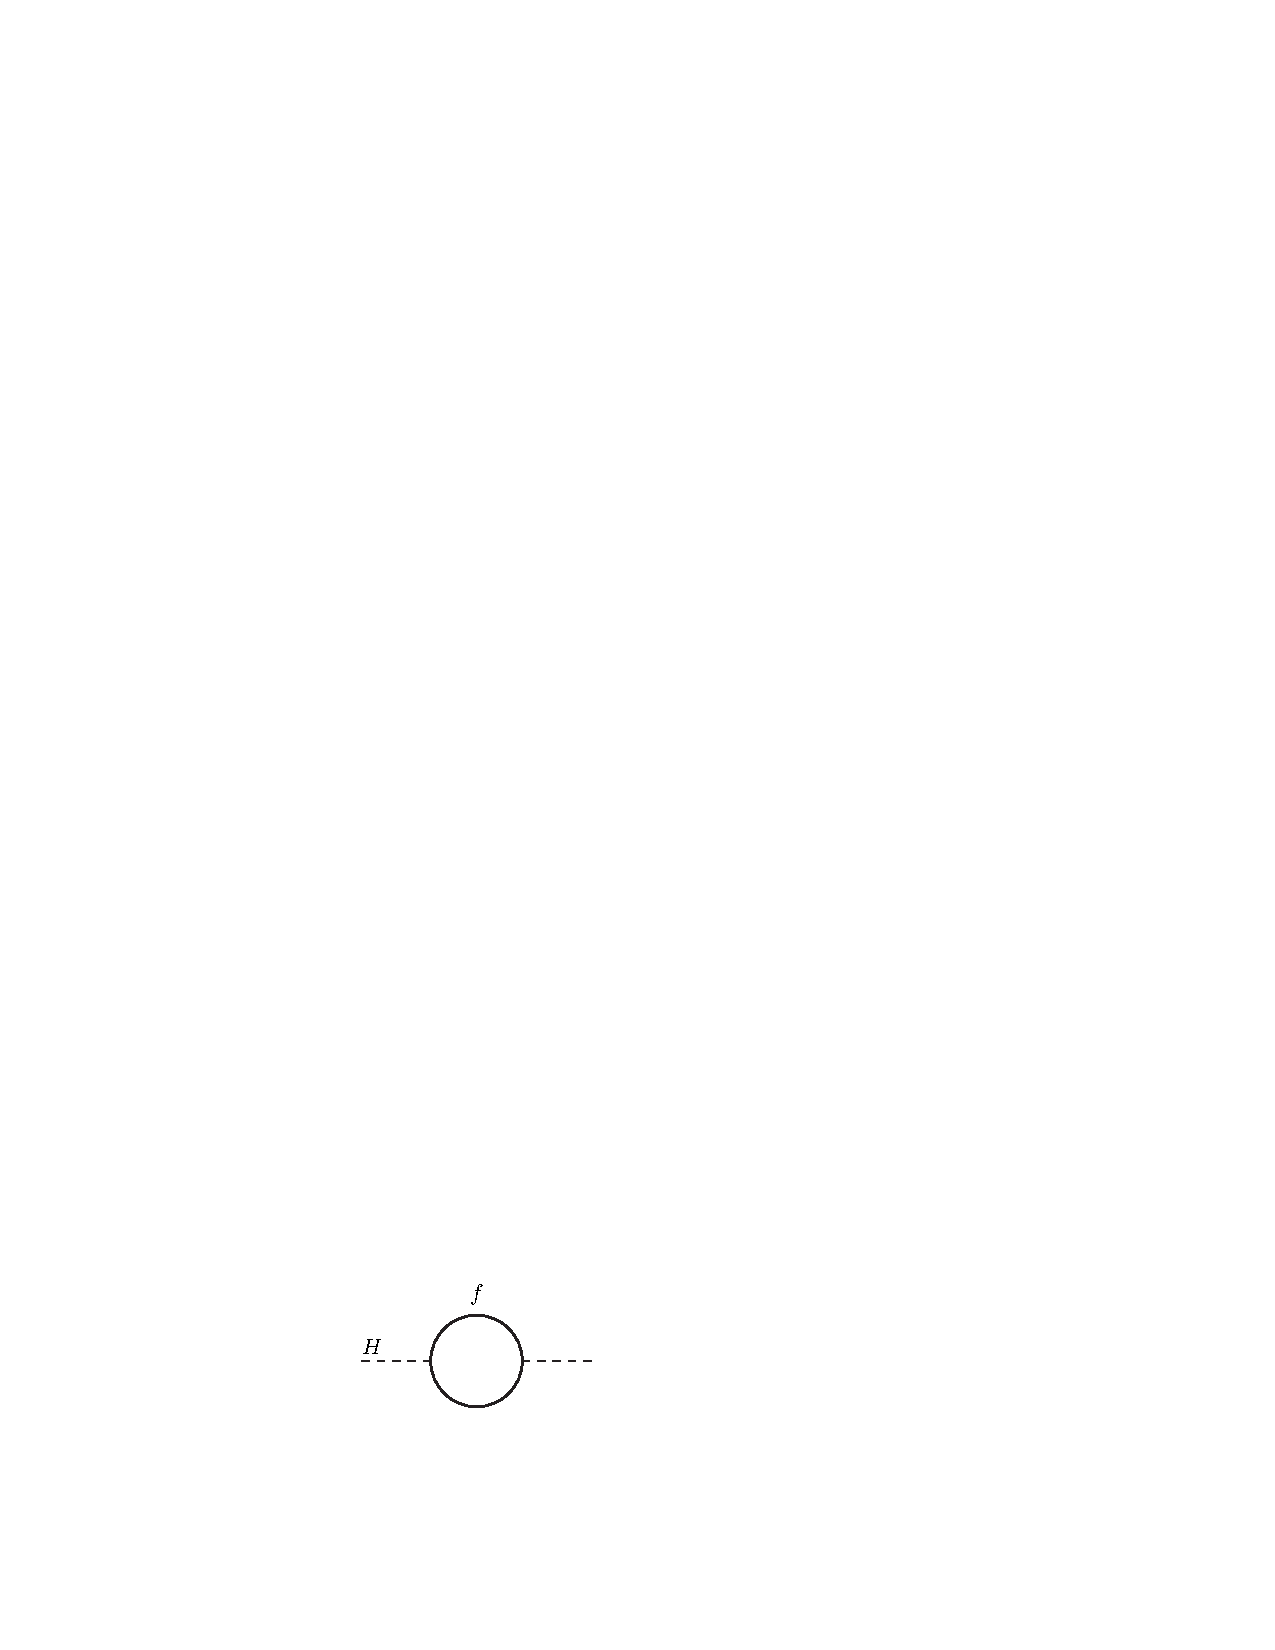
\includegraphics[width=50mm]{figures/theory/HiggsMassCorrection}
  \end{center}
  \caption{Feynman diagram for fermionic loop corrections to the mass of the Higgs boson.}
  \label{img:HiggsMassCorrection}
\end{figure}
The total contribution from these diagrams grows with the cutoff scale of the theory:
\begin{equation}
  \Delta m^{2} = \frac{|\lambda_f|^2}{8\pi^2}\Lambda_{UV}^2 ,
\end{equation}
where $\Delta m^{2}$ is the correction to the higgs mass from a massive fermion, $\lambda_f$ is the coupling constant of the higgs field to that fermion,
and $\Lambda_{UV}$ is the ultraviolet cutoff scale of the theory.
Because the top quark has the largest coupling to the higgs field of the fermions of the Standard Model,
this contribution to the mass of the higgs is dominated by loop corrections involving the top quark.
If one takes $\Lambda_{UV}$ to be the Plank mass (a natural choice for this scale),
then one would expect the Higgs mass to be 30 orders of magnitude larger than it is.
The fact that the Higgs mass is not on the order of the Plank scale is known as the hierarchy problem.
%The hierarchy problem is the implication that in order for the Higgs to have a mass on the order of the electroweak scale,
In order for the Higgs to have a mass on the order of the electroweak scale,
the Standard Model must be extremely fine tuned, as the bare mass of the Higgs boson must be large and negative to
almost exactly cancel contributions from higher order corrections.
%implies that the Standard Model Or that the theory is fine tuned and the bare mass is large and negative almost canceling the correction''
As an alternative to having having a Higgs sector that is extrordinarily finely tuned,
one can introduce new particles that also contribute to the above loop diagrams
and cancel the effect of the Standard Model fermions
or assert that the cutoff scale of the Standard Model is on the order of the Higgs Mass
(meaning, we should expect to see new physics emerge at the Electroweak Scale).
Both of these scenarios gave rise to the hope that new physical theories could be confirmed by the LHC.

A common solution to the hierarchy problem is the introduction of supersymmetric partners to the standard model fermions
that cancel out the standard model fermionic loop corrections to the higgs mass.
However, there exist many non-supersymmetric solutions to the hierarchy problem.
In particular, because the correction to the higgs mass is dominated by a top quark loop,
many of these scenarios introduce new partners to the top quark or new states that couple
strongly to the top quark~\cite{Contino:2008cx,PhysRevD.78.074026,1126-6708-2008-04-087,1126-6708-2009-05-022}.
For this reason, the top quark sector is a promising place to look for new physical signatures.
% T 5/3 and hierarchy problem:
% http://arxiv.org/abs/0801.1679v2


\subsection{Forward Backward Asymmetry}

In addition to the prospect of seeing new physical signatures at the LHC,
recent experimental results have found suggestive deviations from standard model predictions in events involving top quarks.
The validity of these deviations or the existence of models proposed to explain them are testable at the LHC.
The most promising among these results is the measurement of an excess in forward-backward asymmetry in top quark pair production events by both the CDF and D0 experiments.
These experiments both operate on the Tevatron, which is a circular $p-\overline{p}$ collider with a center-of-mass-energy of 1.8 TeV located at Fermilab outside of Chicago, Illinois.
The initial directions of the proton and anti-proton beams can be used to define forward and backward directions,
which are separated by a plane perpendicular to the beam line and going through the beam spot.
To lowest order, the pair production of top quarks is symmetric under interchange of the forward and backward regions.
At tree level in QCD, one does not expect an angular asymmetry in the pair production of top quarks.
However, at higher order, the Standard Model predicts a small forward-backward angular asymmetry that arises from QCD loop corrections \cite{Aaltonen:1318520}.
\begin{figure}
  \begin{center}
    % CDF Paper: http://arxiv.org/abs/1101.0034
    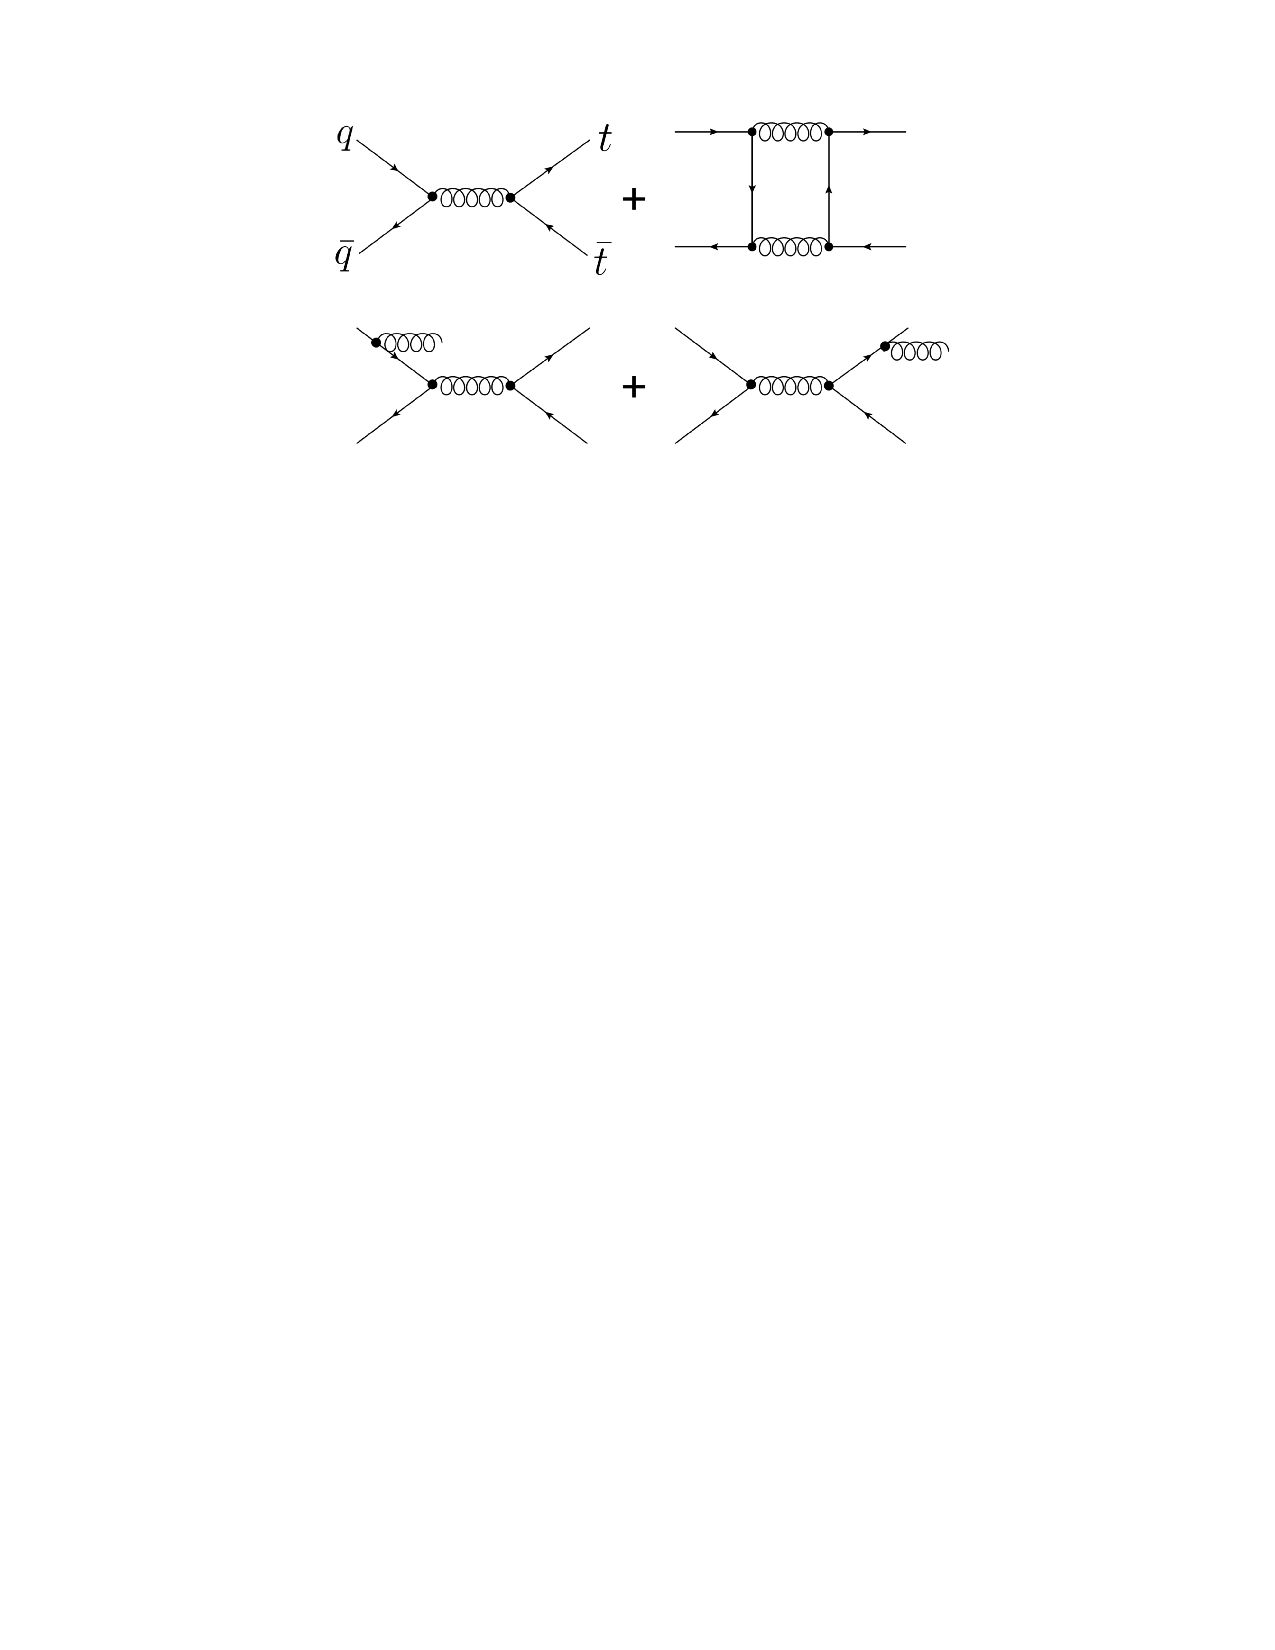
\includegraphics[width=80mm]{figures/theory/ttbarForwardBackwardFeynman}
  \end{center}
  \caption{Feynman diagrams for the pair production of $\ttbar$ in $q-\overline{q}$ collisions.  Asymmetry in the forward-background distribution of the $\ttbar$ system arises from interference between tree-level diagrams and higher-order box diagrams, as seen above.}
  \label{img:ForwardBackwardFeynman}
\end{figure}
This asymmetry can be observed experimentally using an variable that measures the directions of the top quark pairs produced at the Tevatron.
Defining the difference in rapidity between the top and anti-top quarks produced to be $\Delta y = y_{t} - y_{\ttbar}$,
one can measure the number of events with $\Delta y>0$ and $\Delta y<0$, which we refer to as $N(\Delta y>0)$ and $N(\Delta y < 0)$, respectively.
Using these definitions, one constructs the total $\ttbar$ frame asymmetry as
\begin{equation}
  \label{eq:FB_Asymmetry}
  A^{\ttbar} = \frac{N(\Delta y>0) - N(\Delta y>0)}{N(\Delta y>0) + N(\Delta y>0)}
\end{equation}
The standard model prediction for $A^{\ttbar}$ is on the order of $0.06 \pm 0.01$~\cite{Aaltonen:1318520}.
The sign of $\Delta y$ is well-defined at the Tevatron, as one can use the directions of the $p$ and $\bar{p}$ beams to 
define forward and backward regions.
However, at a $p-p$ collider, such as the LHC, the symmetry of the two incoming proton beams prevents one from consistently
defining a sign for $\Delta y$.
% http://arxiv.org/pdf/1101.0034v1.pdf

% [1] L. G. Almeida, G. F. Sterman and W. Vogelsang, Phys. Rev. D 78, 014008 (2008).
% [2] O. Antunano, J. H. Kuhn, and G. V. Rodrigo, Phys. Rev. D 77, 014003 (2008).
% [3] M. T. Bowen, S. D. Ellis, and D. Rainwater, Phys. Rev. D 73, 014008 (2006).
Both CDF and D0 measured this variable using $\ttbar$ events where one top quark decays leptonically and the other hadronically (the single-lepton decay channel).
The presence of the charged final-state lepton can be used to differentiate the top quark from the anti-top quark's decay products.
The selection of hadronic decays on the other quark results in a higher branching ratio than a selection requiring a dileptonically decaying $\ttbar$ system.

Both CDF and D0 see an enhancement in the $\ttbar$ system's forward-backward asymmetry above the small Standard Model prediction.
Of particular interest is the fact that CDF finds this enhancement to increase significantly as a function of the invariant mass of the $\ttbar$ system.
If new physics is responsible for the enhanced forward-backward asymmetry, the invariant mass dependence suggests the deviation from the Standard Model prediction may be the result of interactions with a new massive particle. % http://arxiv.org/abs/1109.3202
To explain the observations, a new particle proposed to address the Tevatron's forward-backward asymmetry must couple strongly
to both first-generation quarks and top quarks and it must couple chirally to produce an asymmetry.

Several categories of models have been proposed~\cite{Almeida:2008,Antunano:2008,Bowen:2006}.
One example is a model of composite light quarks which is enabled by a low Kaluza-Klein scale of extra dimensions~\cite{Delaunay:2011et}.  % KK Excitation: http://arxiv.org/abs/1101.2902
The compositiveness of light, right-handed quarks can lead both to a forward-backward asymmetry as well as an enhancement in the rate of high $p_T$ top quark pairs.
The asymmetry arises from the pair-production of a kk-gluon which subsequently decays into a $\ttbar$ pair, and the decay is asymmetric if there is a large difference between left-handed and right-handed bulk masses.

Other models propose a massive neutral vector boson, or simply Z', which is exchanged via the t-channel by incoming light quarks to produce outgoing top quarks~\cite{Berger:2011vi,Bhattacherjee:2011do}.
%A number of models propose %http://arxiv.org/abs/1109.3202, http://arxiv.org/abs/1102.0545v2,
This process can produce two same-sign top quarks in the final state, which is a rare signature in the Standard Model.

\begin{figure}
  \begin{center}
    % CDF Paper: http://arxiv.org/abs/1101.0034
    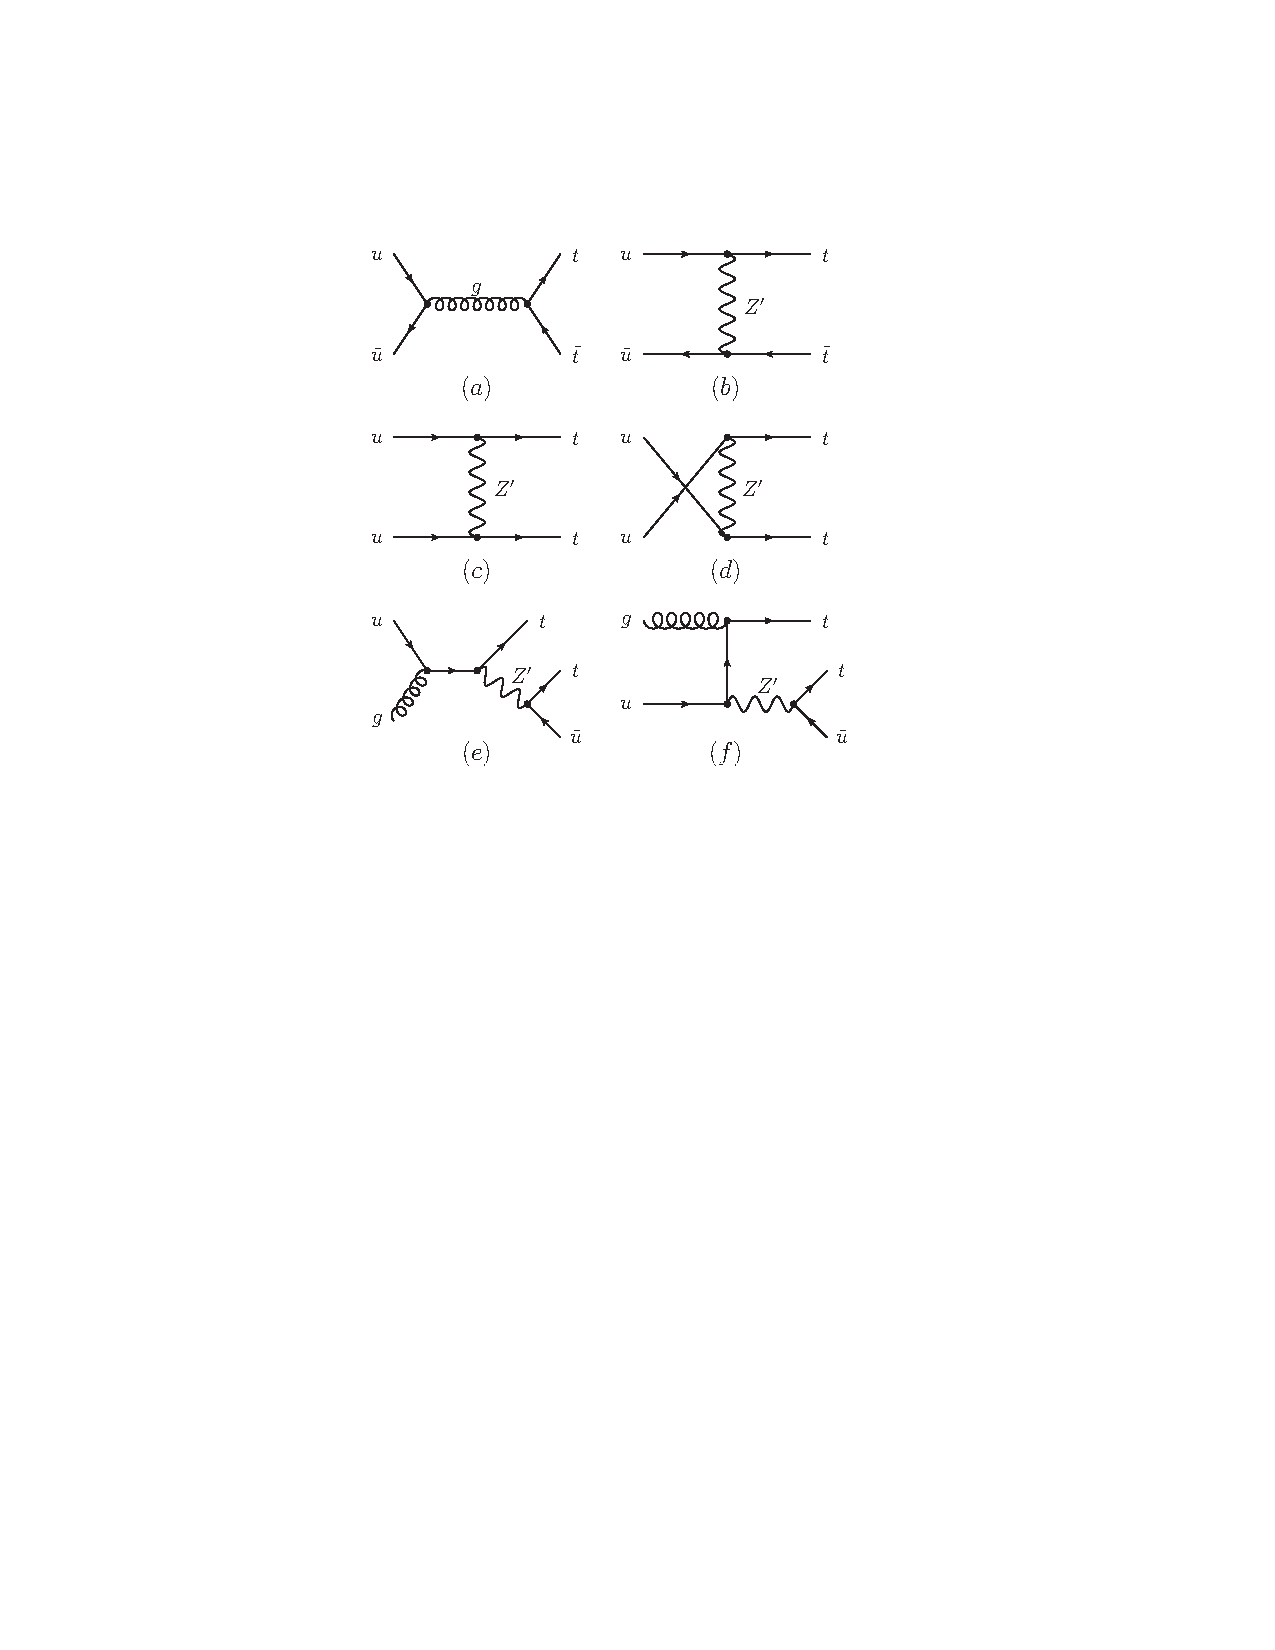
\includegraphics[width=80mm]{figures/theory/AsymmetryZPrimeModel}
  \end{center}
  \caption{Feynman diagrams of contributions to $\ttbar$ production involving a Z'.}
  \label{img:CDFAsymmetryMass}
\end{figure}

%CDF : 20.1 \pm 6.7
%D0 : 19.6 \pm 6.5 % D0 http://arxiv.org/abs/1107.4995

Because the LHC is a proton-proton collider, one cannot define a consistent forward-backward direction in the lab frame (the incoming beam is mirror-symmetric about the collision point).
%% For this reason, directly verifying the tevatron's forward-backward asymmetry anomoly at the LHC requires defining a different discriminating variable than the one used by CDF and D0.
%% Moreover, the larger gluon-gluon contribution to the top pair production cross-section increases the background rate,
%since in the Standard Model and most non-standard models explaining the forward-backward asymmetry,
%the asymmetry occurs among $\ttbar$ events with initial-state quarks. % made up: http://arxiv.org/pdf/0709.1652v1.pdf
%% One can probe this effect at the LHC by measuring a similar variable known as the charge asymmetry.
%% In this quantity, one measures $\Delta|Y| = |y_t| - |y_{\overline{t}} |$ and defines the charge asymmetry to be
%% \begin{equation}
%%   \hat{A}^{\ttbar} = \frac{N(\Delta |y|>0) - N(\Delta |y|>0)}{N(\Delta |y|>0) + N(\Delta |y|>0)}
%% \end{equation}
While this makes the direct measurement of the forward-backward asymmetry at the LHC challenging, there exist techniques for directly probing this effect using modified versions of the discriminating variable defined in equation~\ref{eq:FB_Asymmetry}.
However, equally promising is the prospect of searching for searching for models designed to explain the excess in forward-backward asymmetry observed at the Tevatron.
Several of these models require modifications to the Standard Model that are manifest in the top sector.
For this reason, searches for exotic physical models in the top sector at the LHC are a promising way to explore new physics suggested by this observed excess.
% because direct measurements of the forward-backward asymmetry as observed at the Tevatron are difficult at the LHC, indirect measurements of new physics models designed to explain the forward-backward asymmetry may be more promising.
In particular, many of these models result in same-sign top quark pairs, which can be searched for in regimes that have small backgrounds from the Standard Model, making such searches experimentally appealing.
%These indirect studies include precise measurements of the top quark pair-production cross-section and searches for excesses of events with same-sign top quark pairs.

\subsection{Precision Measurements}
An accurate understanding of the top-quark pair-production cross-section has applications toward understanding particle physics phenomena.
Because top quarks will be produced in large numbers at the LHC, top quark decays are useful for
calibration and validation of the ATLAS detector.
Aside from the direct applications of using the top quark sector to search for new physics,
decays of top quarks are an important background to many analyses throughout analyses conducted by the ATLAS collaboration.
Because the decay of top quarks lead to a wide range of final states, they appear as backgrounds to
numerous search channels for the Higgs boson, many Super Symmetry analyses, and across a wide range of exotic searches.

%A good example is a recent analysis which uses the \ttbar cross-section to constrian the gluon parton distribution function. % http://arxiv.org/abs/1303.7215

% However, because the The early measurements at the LHC d

%% % CDF Subsection
%% \subsection{CDF}

%% The CDF collaboration tagged $\ttbar$ events using the following event selection:
%% \begin{itemize}
%%   \item 1 selected lepton with $E_T \ge 20$ GeV and $| \eta | <$ 1
%%   \item 4 hadronic jets with $E_T  > 20$ GeV and $| \eta | <$ 2
%%   \item $\met >$ 20 GeV
%% \end{itemize}

%% The choice of jets to associate with the hadronically decaying top was made using a $\chi^2$ kinematic fit to the full $\ttbar$ system using the mass of the W-bosons and top quarks as constraints and assigning b-tagged jets, if any, to b quarks at the parton level.
%% Expected signal and background distributions were evaluated using PYTHIA Monte-Carlo simulation.

%% The CDF measurement found a forward-backward asymmetry of $A = 0.150 \pm 0.055$ (stat+sys), which is two standard deviations away from the predicted value from NLO simulations.
%% In addition, the significance of this deviation was examined as a function of both the difference in rapidity ($Y$) and the invariant mass of the $\ttbar$ system:

%% % From Here: http://arxiv.org/pdf/1101.0034v1.pdf
%% % Page 13: http://arxiv.org/abs/1101.0034
%% \begin{tabular}{lcc}
%% Selection                         &   CDF Result    & SM Prediction \\
%% $A^{\ttbar}_{FB}( \Delta Y < 1.0)$  & 0.026 $\pm$ 0.118 & 0.039 $\pm$ 0.006 \\
%% $A^{\ttbar}_{FB}( \Delta Y > 1.0)$  & 0.611 $\pm$ 0.256 & 0.123 $\pm$ 0.008 \\
%% \hline
%% $A^{\ttbar}_{FB}( M_{\ttbar} < 450 GeV)$   & -0.116 $\pm$ 0.153 & 0.040 $\pm$ 0.006 \\
%% $A^{\ttbar}_{FB}( M_{\ttbar} \ge 450 GeV)$ & 0.475 $\pm$ 0.114  & 0.088 $\pm$ 0.013 \\
%% \hline
%% \end{tabular}

%% Of note is the fact that the deviance of the asymmetry from prediction is a function of the invariant mass of the $\ttbar$ system.

%% \begin{figure}
%%   \begin{center}
%%     % CDF Paper: http://arxiv.org/abs/1101.0034
%%     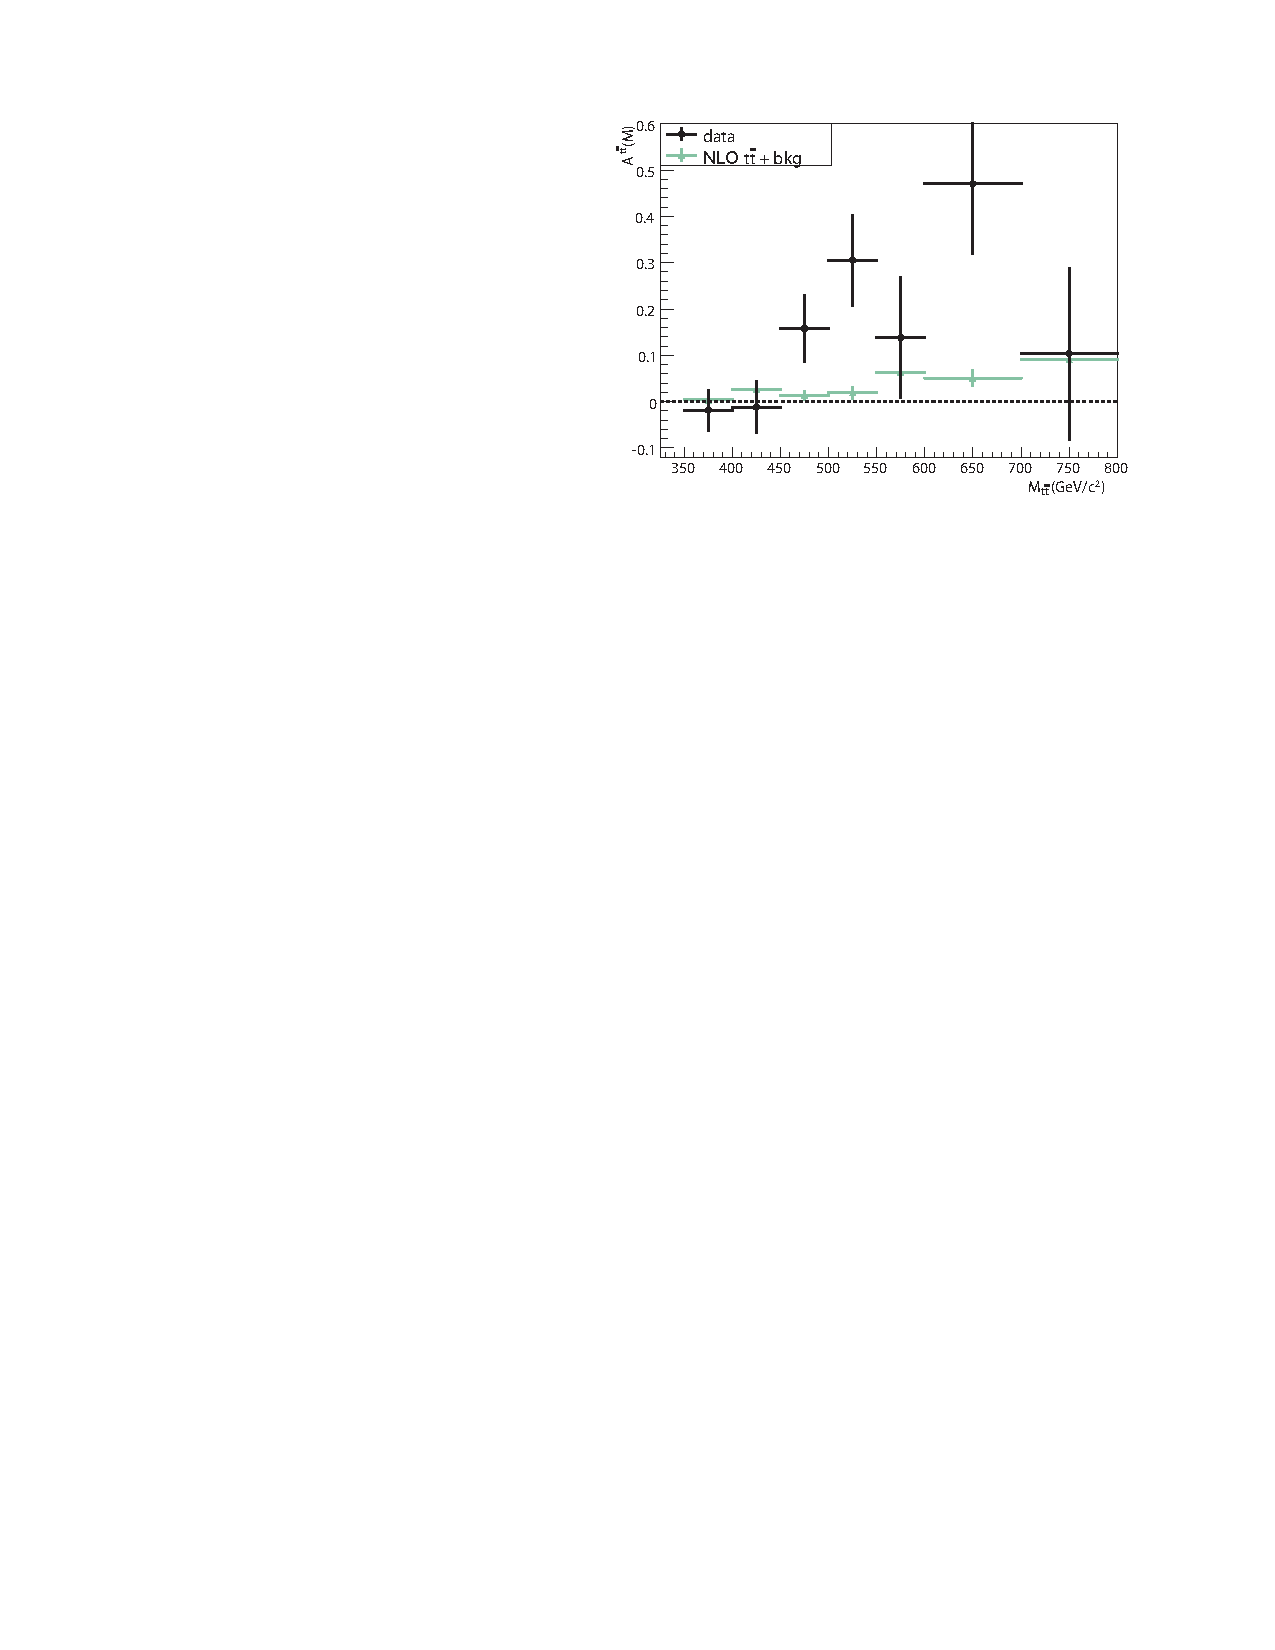
\includegraphics[width=80mm]{figures/theory/CDFAsymmetryMass}
%%   \end{center}
%%   \caption{Graph of the forward-backward asymmetry as a function of the invariant mass of the $\ttbar$ system.}
%%   \label{img:CDFAsymmetryMass}
%% \end{figure}


%% % D0 Subsection
%% \subsection{D0}

%% The D0 experiment selected $\ttbar$ events by triggering on either a lepton or a lepton+jet and further requiring
%% \begin{itemize}
%%   \item An isolated lepton with $p_T >$ 20 GeV and $|\eta| <$ 1.1 for electrons or $|\eta| <$ 2.0 for muons
%%   \item $\met >$ 20 GeV for electron events or $20 GeV < \met < 250 GeV$ for muon events
%%   \item $\Delta \phi(e, \met) > (2.2 - 0.045*\met / GeV)$ radians for electron events or $(p_T^\mu + \met)^2 - (p_x^\mu + \met_x)^2 - (p_y^\mu + \met_y)^2 < (250 GeV)^2$
%%   \item 4 jets, each with $pt > 20 GeV$ and $|\eta < 2.5|$ where the leading jet has $p_t > 40 GeV$
%% \end{itemize}

%% D0 measured an overall forward-backward asymmetry of $(9.2 \pm 3.7)$\%, where the predicted value is $(2.4 \pm 0.7)$ \%.

%% \begin{tabular}{lcc}
%% \hline
%% Selection                         &   CDF Result    & SM Prediction \\
%% \hline
%% $A^{\ttbar}_{FB}( \Delta Y < 1.0)$ &   6.1 $\pm$ 4.1 & 1.4 $\pm$ 0.6 \\
%% $A^{\ttbar}_{FB}( \Delta Y > 1.0)$ &  21.3 $\pm$ 9.7 & 6.3 $\pm$ 1.6 \\
%% \hline
%% $A^{\ttbar}_{FB}( M_{\ttbar} < 450 GeV)$ & 7.8 $\pm$ 4.8 & 1.3 $\pm$ 0.6 \\
%% $A^{\ttbar}_{FB}( M_{\ttbar} \ge 450 GeV)$ & 11.5 $\pm$ 6.0 & 4.3 $\pm$ 1.3 \\
%% \hline
%% \end{tabular}

%\subsection{Discussion}

% LocalWords:  Higgs
